\documentclass[screen,review]{acmart}
\usepackage{makecell} % Include the makecell package

\AtBeginDocument{%
  \providecommand\BibTeX{{%
    Bib\TeX}}}

\setcopyright{acmlicensed}
\copyrightyear{2024}
\acmYear{2024}

\begin{document}

\title{EHRAgent Reproduction and Extension}

\author{Peter Iat Kei Ho}
\email{peter-ho@live.com}
\affiliation{
  \institution{University of Texas, Austin}
  \city{Austin}
  \state{Texas}
  \country{USA}
}

\renewcommand{\shortauthors}{Peter Ho}

\begin{abstract}
  Even though EHRAgent based on gpt4 was proven to have better result 
  than other solution by the work this report is based on, There are 
  still many challenges in reproduction and optimization.
\end{abstract}

\begin{CCSXML}
  <ccs2012>
     <concept>
         <concept_id>10010405.10010444.10010447</concept_id>
         <concept_desc>Applied computing~Health care information systems</concept_desc>
         <concept_significance>500</concept_significance>
         </concept>
     <concept>
         <concept_id>10011007.10011074.10011099.10010876</concept_id>
         <concept_desc>Software and its engineering~Software prototyping</concept_desc>
         <concept_significance>500</concept_significance>
         </concept>
     <concept>
         <concept_id>10002951.10002952.10003197.10010822.10010823</concept_id>
         <concept_desc>Information systems~Structured Query Language</concept_desc>
         <concept_significance>300</concept_significance>
         </concept>
     <concept>
         <concept_id>10010147.10010257.10010282.10010291</concept_id>
         <concept_desc>Computing methodologies~Learning from critiques</concept_desc>
         <concept_significance>300</concept_significance>
         </concept>
     <concept>
         <concept_id>10010147.10010257.10010258.10010259.10003343</concept_id>
         <concept_desc>Computing methodologies~Learning to rank</concept_desc>
         <concept_significance>100</concept_significance>
         </concept>
   </ccs2012>
\end{CCSXML}
  
\ccsdesc[500]{Applied computing~Health care information systems}
\ccsdesc[500]{Software and its engineering~Software prototyping}
\ccsdesc[300]{Information systems~Structured Query Language}
\ccsdesc[300]{Computing methodologies~Learning from critiques}
\ccsdesc[100]{Computing methodologies~Learning to rank}

\keywords{EHR, Agent, LLM, Azure, OpenAI, Python, Debug, SQL, MIMIC }

\maketitle

\section{Introduction}
According to \url{https://www.thebalancemoney.com/causes-of-rising-healthcare-costs-4064878}, 
cost of healthcare has significantly increased over past decades and years, which can be a 
risk for health and well being of Americans impacting every age group. I believe there 
are many factors with many different solutions. One of them is leveraging technology 
to help medical professionals to focus their time and energy on patients and/or research 
but not simple data retrieval or analysis.

LLM (Large Language Model) has gained signficant popularity over the past years. It can 
capture semantics of text, memorize past conversations, and generate code. This report 
evaluates past work that utilizes MIMIC\cite{PhysioBank_PhysioToolkit_PhysioNet}\cite{physioNet}\cite{Johnson2016}
dataset by reproducing and considering alternatives in data retreival and analysis.

\section{Related Work}
This a reproduction and alternation of part of the work - ["EHRAgent: Code Empowers Large Language Models 
for Complex Tabular Reasoning on Electronic Health Records"]\url{https://arxiv.org/abs/2401.07128}. 
EHRAgent is an LLM agent empowered with a code interface, to autonomously generate and 
execute code for complex clinical tasks within electronic health records (EHRs). 
The original project page is available at [this link](https://wshi83.github.io/EHR-Agent-page/). \cite{shi2024ehragent}

Text to SQL generation is another related project that the former utilizes its evelation logic 
with slight modification. Information of the project can be found at
\url{https://github.com/wangpinggl/TREQS/blob/master/README.md} \cite{wang2020text}

\section{Methodology}
\begin{figure}[h] 
  \centering
  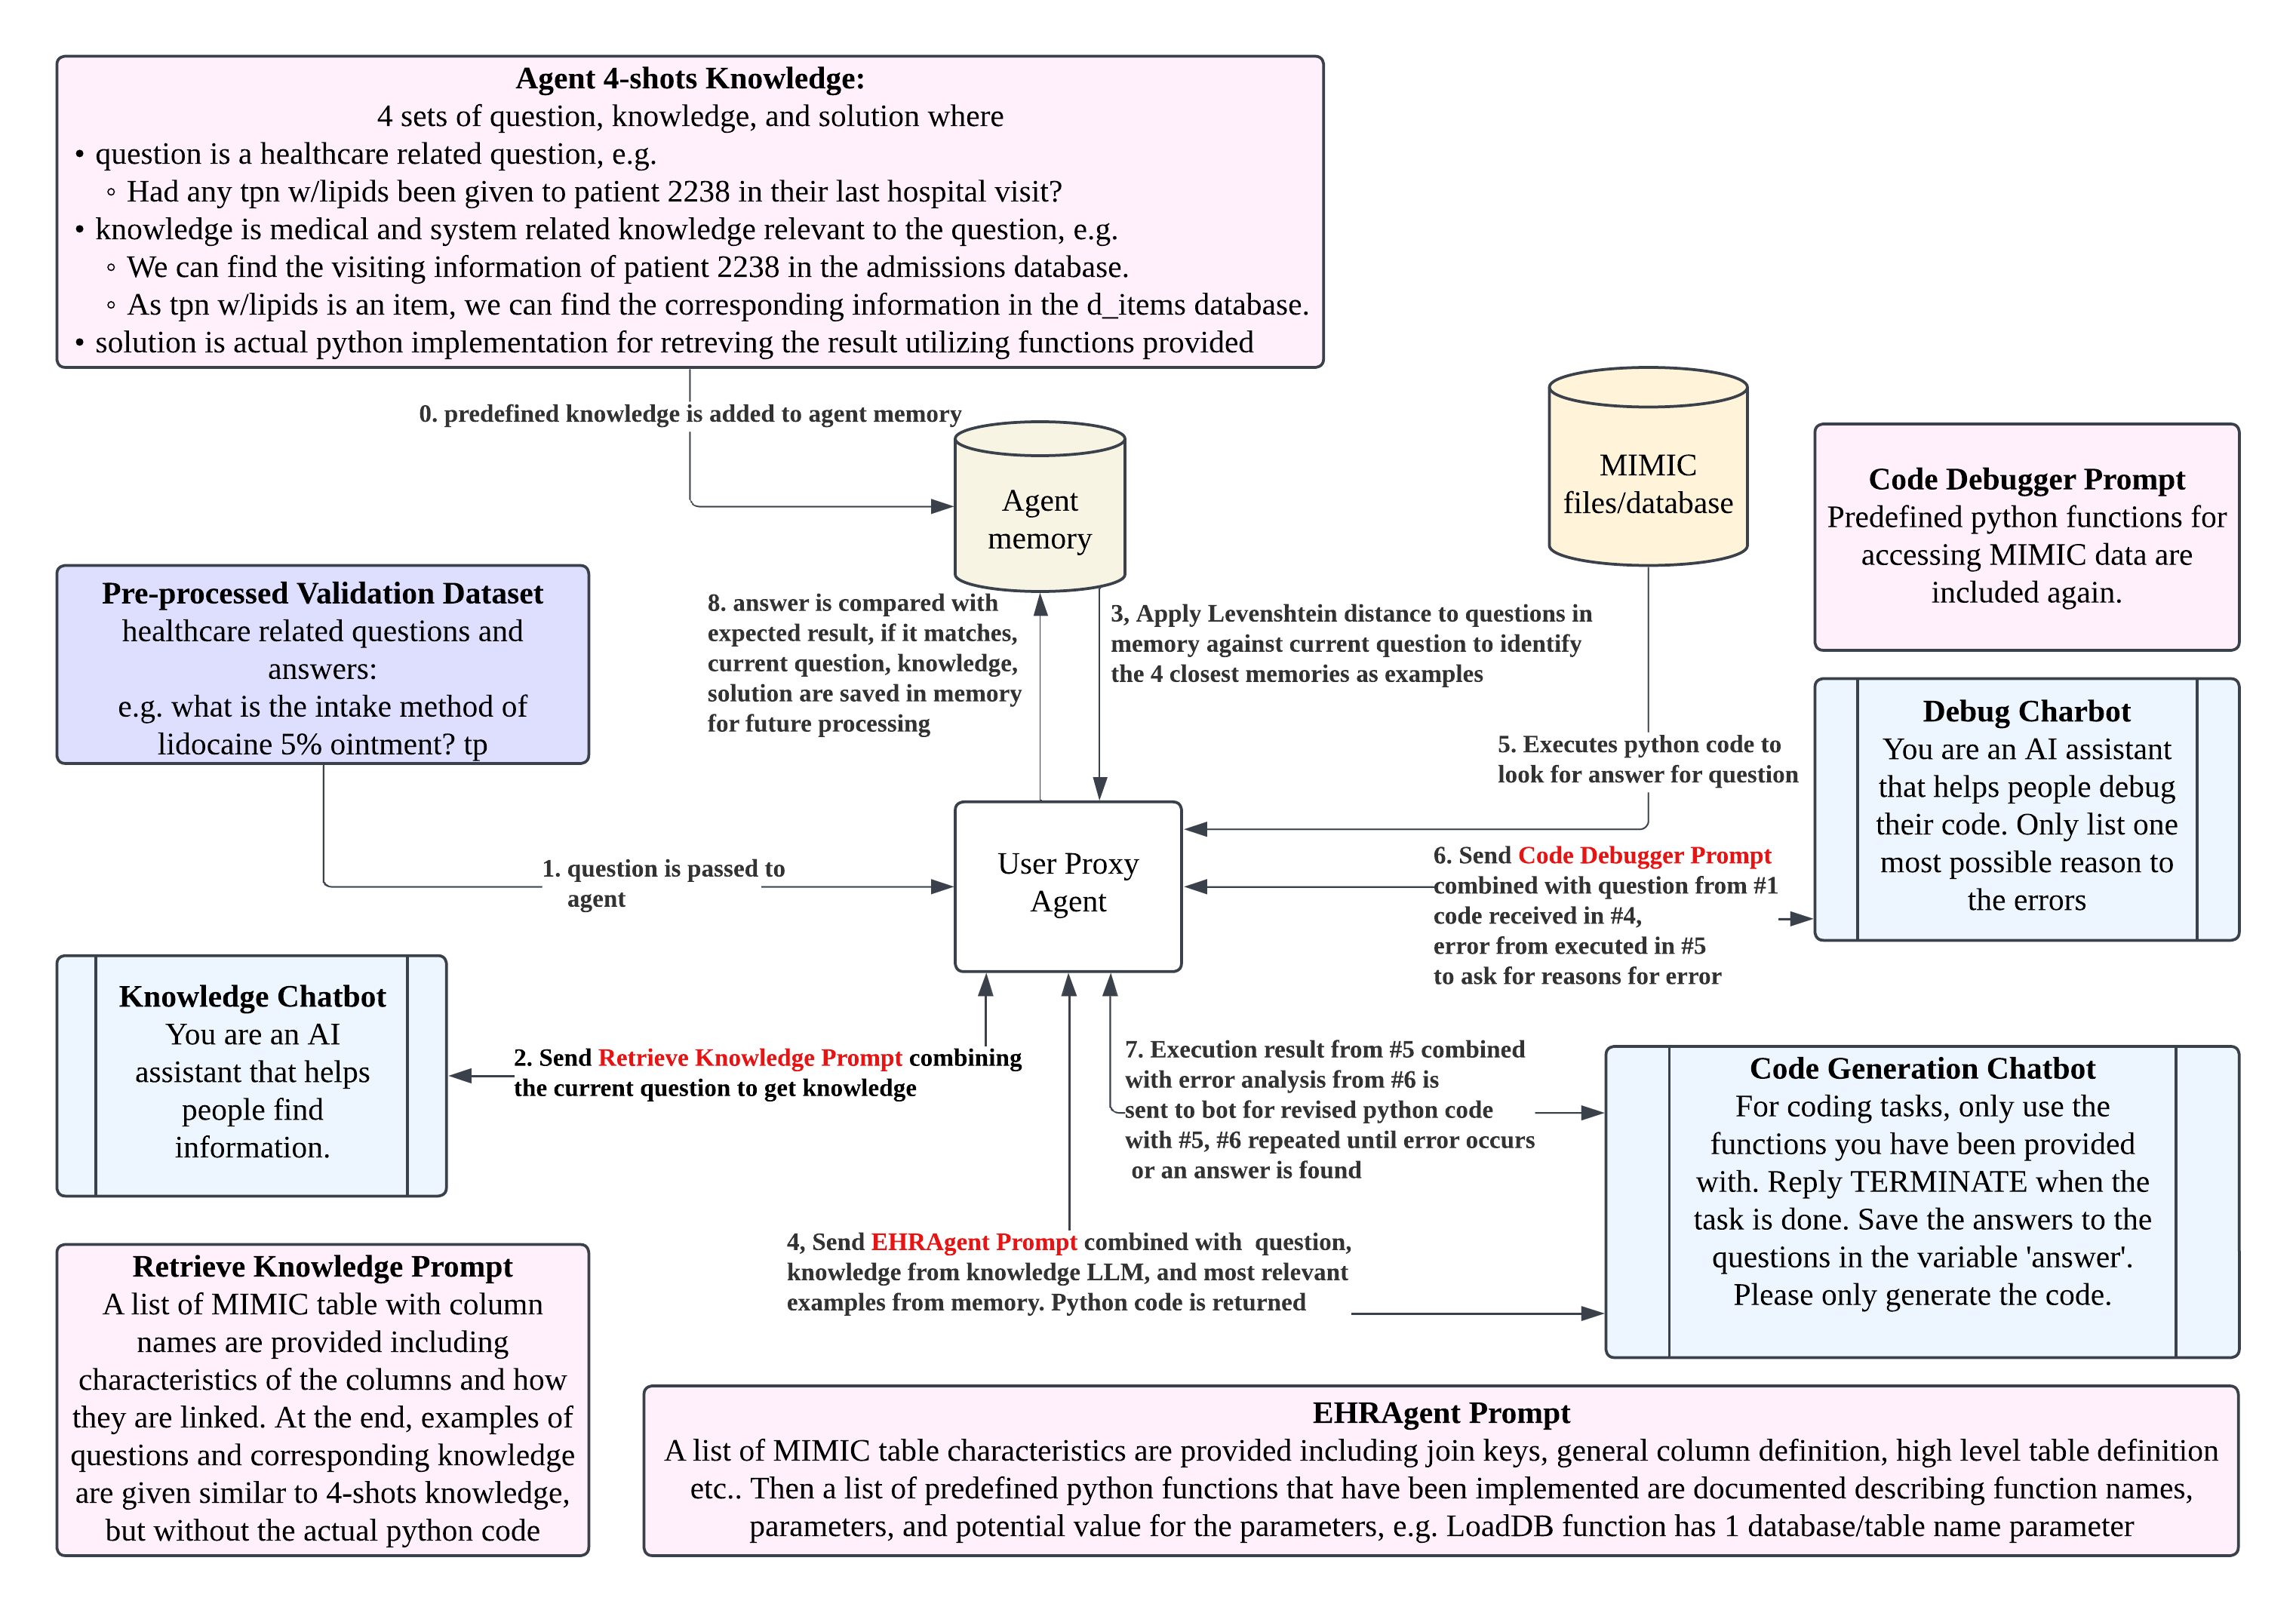
\includegraphics[width=\textwidth]{ehragent.png}
  \caption{EHRAgent execution flow}
  \Description{This diagram illustrates execution flow of EHRAgent 
  describing each step from initializing memory, 
  to get question for processing, to having various 
  chatbots to answer the question}
  \label{fig:ehragent}
\end{figure}

\subsection{Agent Execution Steps}
\begin{enumerate}
  \setcounter{enumi}{-1}
  \item Predefined knowledge is intialized as memory, including question, knowledge, and associated solution.
  \item A question from validation data set is passed into UserProxyAgent 
  \item During initialization process of main code generation chat, UserProxyAgent sends question to Knowledge 
  chatbot to retrieve knowledge regarding the question applying chain of thought. Few shot learning is also 
  applied as the prompt to the knowledge chatbot includes examples of questions and their corresponding knowledge. 
  \item Retrieve 4 most similar examples by comparing current question with questions in memory according to 
  levenshtein distance, applying few shot learning.
  \item Invoke code generation chatbot with table definition, function definition, knowledge retrieved from 
  knowledge chatbot, examples from memory.
  \item Execute code retrieved from bot and identify answer or errors. IF errors were encountered, 
  capture errors and provide potential hints in resolving them.
  \item When error was thrown in the last step, functions documentation, code executed and execution error 
  are sent to debugger chatbot to identify potential fixes.
  \item Original error message and suggestions returned by debugger chatbot are packaged as response back to 
  code generation cahtbot for it to review and regenerate a better response. As chat with code generation 
  chatbot continues until error occured related to exceeding max token size or termination message was identified.
  \item The response is then compared with predefined answer, if the answer was correct, the question, knowledge 
  and solution are all stored in memory for future reference.
\end{enumerate}

\subsection{Original functions provided for chatbot}
\begin{enumerate}
  \item{\texttt{Calculate}}: passes argument to wolfram alpha for mathematical calculation.
  \item{\texttt{LoadDB}}: loads a MIMIC csv file into memory
  \item{\texttt{FilterDB}}: filters data returned froom LoadDB with predefined common operators similar to SQL WHERE clause, 
  but with a little more functionality including min and max, which selects the row equals to the minimum or maximum of the whole file. 
  \item {\texttt{GetValue}}: retrieves a string based on a comma delimited list of column names 
  provided in table definition, with some operator supported including sum.
  \item {\texttt{SQLInterpreter}}: executes a given sql against sqlite3 database.
  \item {\texttt{Calendar}}: evaluates the date after the duration of time based on sqlite3 database
  datetime function referencing current\_time
\end{enumerate}

\subsection{Issues regarding original work}
\begin{enumerate}
  \item{\texttt{Cost}}: The table cost was referenced in multiple places of the original implementation including examples, 
  validaton questons and answers, but in MIMIC-III v1.4, cost is not a file available for download, nor in the demo dataset. 
  Any question related to cost can't be answered, and solution based on the example referring to cost would result in 
  a table not found error, which can't be recovered.
  \item{\texttt{Python Package dependency}}: In requirements.txt, autogen version 1.0.16 was referred, but 0.3.2 is the latest 
  when this report was written. 0.3.3 was released afterwards, but it's still quite far from 1.0.16.
  \item{\texttt{Sqlite3 calendar calculation}}: After setting up sqlite3 by importing MIMIC-III v1.4 csv files, 
  sqlite3 database datetime function doesn't use current date even though current\_time was passed in. 
  It used 2000-01-01, so with input of -1 day, 1999-12-31 was returned.
  \item{\texttt{LoadDB requirement}}: Since LoadDB reads the whole table into memory, for larger table, 
  out of memory exception was thrown. Due to re-reading the same csv or csv.gz files for every LoadDB command
  for various questions, disk IO can cause unnecessary delays when reading against the same data.
  \item{\texttt{Validation set issue}}: When trying to identify reasons for incorrect responses, SQL embedded in the validation
  data set was used to identify and verify given answers. There are answers that are incorrect based on data retrieved from MIMIC-III v1.4. 
  \item{\texttt{Execution challenge}}: Since some code generated by chatbot can be quite inefficient, there are times that it 
  takes more than hours to run, and sometimes it can be hard to tell how long it will take for the process to terminate. 
  So with more than 500 validation questions, it takes more than days to finish evaluating 1 implementation.
\end{enumerate}

\subsection{Adjustments}
\begin{enumerate}
  \item{\texttt{Cost}}: Since examples related to cost won't be relevant and validation questions related to 
  cost will not work, 24 questions and answers involving costs were removed. Examples related to costs were 
  also adjusted to better illustrate other implementation.
  \item{\texttt{Python Package dependency}}: Autogen 0.3.2 was used instead of 1.0.16, flaml[automl] 
  was added due to other dependency. And mariadb 1.1.11 was added to support accessing MariaDB.
  \item{\texttt{Sqlite3 calendar calculation}}: Calendar calculation was changed to MariaDB DATE\_ADD which 
  evaluates duration based on current datetime instead of 2000.
  \item{\texttt{LoadDB requirement}}: LoadDB and several other functions are changed to defer execution 
  similar to Apache Spark, so only result after filtering and selected columns is returned and read from data source.
  \item{\texttt{Execution challenge}}: Due to the time sensitive nature of this report, when the evaluation of a question 
  takes more 45 minutes, the process is killed with question id marked as not complete and restarted.
  \item{\texttt{Database backend}}: To help improve data operations, instead of loading from files every time, 
  all operations invokes MariaDB backend with database indexes setup for larger tables. 
  \item{\texttt{New functions}}: Given database operations aren't as straightforward to be mapped with 
  results returning multiple values or list when only one value is needed, new functions are added 
  including GetValue getting a single, GetValues getting multiple values, 
  GetCount count the number of rows of a data set.
\end{enumerate}

%%Result - Outline your major results. Tell your readers about the impact or usefulness of what you discovered.
\section{Result}
\begin{table}[H]
  \centering
  \caption{Execution result}
  \label{tab:result}
  \centering
  \begin{tabular}{|c|c|c|c|}
      \hline
       & \makecell{\textbf{Number of} \\ \textbf{Question}} & \makecell{\textbf{Success} \\ \textbf{Rate}} & \makecell{\textbf{Completion} \\ \textbf{Rate}}  \\
      \hline
      \makecell{\textbf{EHRAgent} \\ from original \\ work\cite{shi2024ehragent} } & 581 & 53.10 & 91.72\\
      \hline
      \makecell{\textbf{EHRAgent} \\ \textbf{w/o cost}} & 556 & 26.08 & 69.96\\ 
      \hline
      \makecell{\textbf{EHRAgent with} \\ \textbf{MariaDB w/o cost}} & 556 & 26.08 & 69.96\\
      \hline
  \end{tabular}
\end{table}
Since the cost file is not available and some of the question's ground-truth answer is incorrect after verifying by the provided SQL 
against MIMIC data, I believe it's likely that the dataset of the original work\cite{shi2024ehragent} is different from the MIMIC 
data set used in this report. With the result being comparable between EHRAgent and EHRAgent with MariaDB, the code generation 
has not improved even though some new functions are provided. But the amount of time it took to finish processing the full set of 
questions has improved quite a bit. Due to the process being randomly crashed and processing of some questions were killed inconsistently
, duration of processing was not accurately captured. But the amount of time it took to finish without MiraDB was signiificantly larger
than the processing with MiraDB. 

\section{Conclusion}
%%Conclusion - Summarize your project. Then, point out the future directions or things can be improved or expanded upon in the future.
EHRAgent\cite{shi2024ehragent} promised significant improvement comparing to related work. This report attempts to reproduce it, 
evaluate problems during the process, and make adjustments to the solution. But even though the dataset 
mentioned being MIMIC-III, the dataset doesn't seem to match the MIMIC-III dataset available on PhysioNet - 
\url{https://physionet.org/content/mimiciii/1.4/} which caused a big difference between the original result and reproduced results. 

Even though improved solution with MariaDB took signficantly less time, correction rate and completion rate were the same. 
I believe incorrect ground truth can also caused this correction rate to be lower than expected in both evaluation. 
Potential next steps can be:  
\begin{itemize}
  \item having a set of verification questions and ground truth answers matching the test data.
  \item adjusting initial memory so they are more diverse.
  \item persisting memory captured by answering questions correctly so that when the process hangs and needs to be destroyed, memory can be recovered.
  \item providing more robust filtering examples, as some generated code has applied multiple filtering which can be incorrect in some cases.
\end{itemize}

\bibliographystyle{ACM-Reference-Format}
\bibliography{report}

\end{document}
\endinput
